\section{Liturgia chrzcielna}

\subsection{Procesja do baptysterium}

\begin{itemize}
	\item podczas ostatniego proroctwa:
	      \begin{itemize}
		      \item \aa\aa~ odpalają akolitki od znicza
		      \item \ding{63} idzie po krzyż procesyjny
		      \item \paschal~ idzie do Paschału \footnote{Paschał stoi na
			            stojaku poza prezbiterium} i go odpala \footnote{Można
			            to zrobić cieńką, woskową świeczką od znicza}
	      \end{itemize}
	\item po ostatniej oracji:
	      \begin{itemize}
		      \item kantorzy \underline{niezłowcznie}
		            podejmują śpiew \textit{Sicut Cervus}
		      \item \ii, \dd, \ss~ z \cc1 schodzą krótką drogą do sedilli,
		            \ii~ ściąga \textcolor{violet}{fioletowy ornat i manipularz}
		            (pomaga \zz~ \footnote{Orant zostaje wyniesiony do zakrystii
			            -- na Mszy będzie używany ornat \textcolor{red}{czerwony}})
		            i wkłada \textcolor{violet}{fioletową kapę} (pomaga \cc1)
		      \item \dd~ i \ss~ ściągają \textcolor{violet}{fioletowe manipularze}
		      \item \cc1 bierze birety
		      \item formuje się procesja (nadzoruje \cc2)
		            \begin{center}
			            \dd~~~\ii~~~\ss \smallskip\\
			            \cc1 \\
			            ministranci \smallskip\\
			            kantorzy \smallskip\\
			            \aa1~~~\ding{63}~~~\aa2 \smallskip\\
			            \cc2~~\paschal~~~~~~~ \smallskip\\
			            $\downarrow$
		            \end{center}
	      \end{itemize}
	\item procesja rusza na znak \cc1 (patrz Rys. \ref{fig:procesja1})
\end{itemize}
%
\begin{figure}[h]
	\centering
	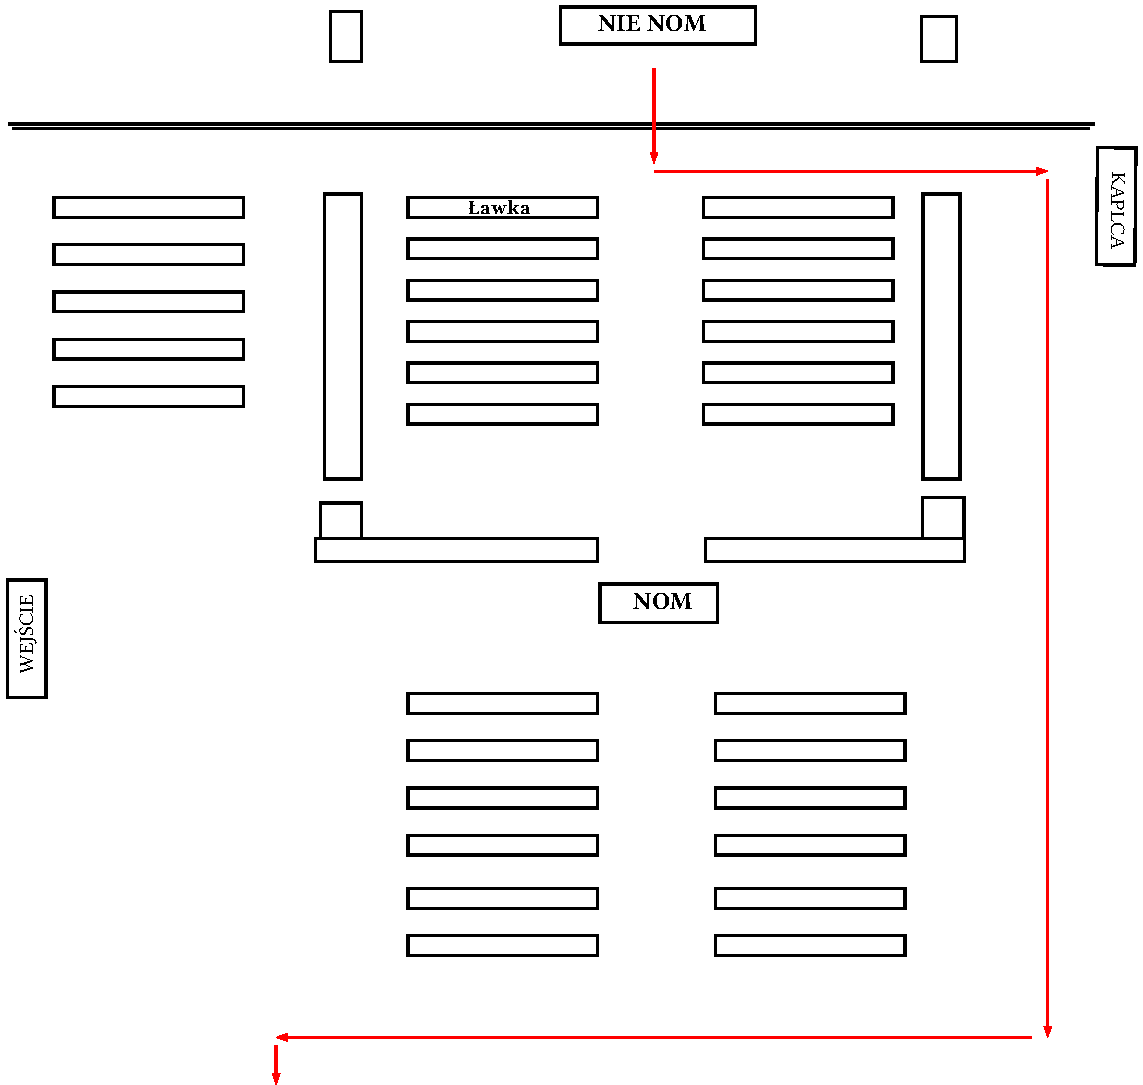
\includegraphics[width=0.55\linewidth]{procesja1.pdf}
	\caption{Droga do chrzcielnicy}
	\label{fig:procesja1}
\end{figure}
%
\subsection{Poświęcenie wody}
\begin{itemize}
	\item po dojściu do kraty:
	      \begin{itemize}
		      \item ministranci funkcyjni wchodzą do baptysterium (patrz Rys.
		            \ref{fig:woda})
		      \item chór też wchodzi do baptysterium, ale głębiej (koło drzwi
		            wejściowych) \footnote{Zostawiając przy tym miejsce dla
			            chóru, który musi stać bliżej chrzcielnicy} (patrz Rys.
		            \ref{fig:woda})
		      \item \ii, \ss, \dd~ i \cc2 stoją przed kratą (jeszcze nie patrz
		            Rys. \ref{fig:woda})
	      \end{itemize}
	\item \ii~ ściąga biret, podaje \dd~ a ten \cc1, \cc1 odnosi i przynosi
	      księgę z modlitwą. \ii~ czyta kantyk \textit{Sicut Cervus} i czeka, aż
	      chór skończy jego śpiewanie. Następnie odczytuje oracje
	      \smallfont{(złożone ręce)} i po jej skończeniu wchodzi do baptysterium
	      (teraz patrz Rys. \ref{fig:woda})
	      \begin{figure}[h!]
		      \centering
		      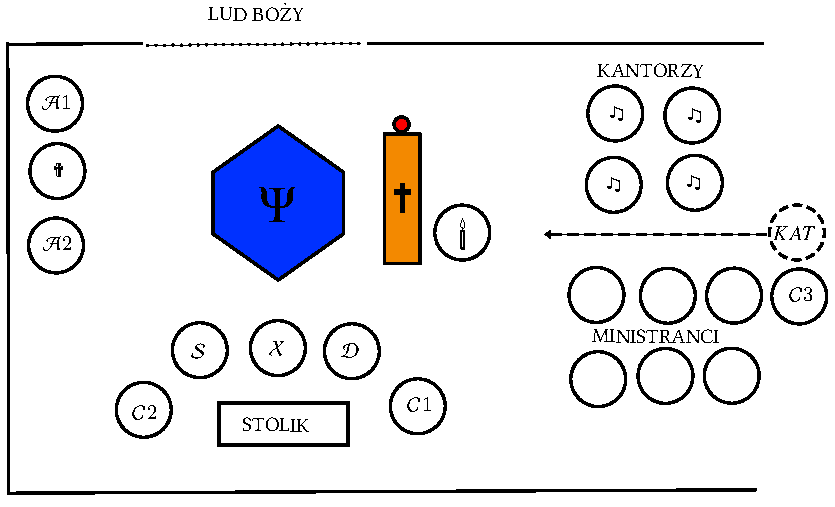
\includegraphics[width=0.7\linewidth]{woda.pdf}
		      \caption{Ustawienie przy chrzcielnicy, \spiew~ oznacza kantorów,
			      $KAT$ oznacza katechumena}
		      \label{fig:woda}
	      \end{figure}
	\item następuje poświęcenie wody chrzcielnej, \dd~ i \ss~ podtrzymują brzegi
	      kapy i pomagają \ii~ podając odpowiednie rzeczy (oleje, ręcznik
	      \dots), które podstawia \cc1
	      (patrz \textit{\nameref{sec:woda}})
\end{itemize}
\subsection{Chrzest}
\begin{itemize}
	\item \ii~ zmienia {\color{violet} fioletową kapę i stułę} na
	      \textcolor{black!50}{białą kapę i stułę}, \dd~ i \ss~ pozostają w
	      szatach \textcolor{violet}{fioletowych}
	\item \cc3 wprowadza do baptysterium katechumenów z chrzestnymi (stoją oni
	      za ministrantami i kantorami)
	\item katechumeni stają po przeciwnej stronie chrzcielnicy od Paschału, obok
	      \ss
	\item \ii~ rozpoczyna dialog z katechumenami
	\item po odpowiedziach na wszystkie pytania, \ii~ nad chrzcielnicą
	      trzykrotnie polewa głowę dziecka lub dorosłego, wypowiadając formułę
	      chrzcielną
	\item \cc1 podaje \dd~ naczynie z Krzyżmem, a \dd~ podaje \ii. \ii~
	      namaszcza ochrzczonych wypowiadając formułę i wyciera kciuk w watę
	\item następnie wręcza się białą szatę oraz płonącą świecę, wypowiadając
	      przepisane formuły
	\item następnie \ii~ wypowiada formułę: \textit{N., vade in pace...}
\end{itemize}
\subsection{Bierzmowanie}
\begin{itemize}
	\item kantorzy podejmują śpiew \textit{O stworzycielu Duchu Przyjdź}
	      % \item wszyscy oprócz \ii, \cc1, \cc2, \cc3 i \cc4 oraz \paschal~
	\item wszyscy (oprócz \paschal) wychodzimy procesyjnie z baptysterium i
	      idziemy w stronę kaplicy św. Iwa
	\item \ii, \dd, \ss, \cc1, \cc2 wchodzą do kaplicy a reszta procesji idzie
	      kawałek za kaplicę i staje jak na Rys. \ref{fig:bierzmowania}
	\item w kaplicy
	      \begin{itemize}
		      \item \ii~ staje przy faldistorium
		      \item \dd~ i \ss~ stoją po bokach \ii~ i podtrzymują kapę
		      \item \cc1 bierze księgę z kredencji i podchodzi do \ii~
		      \item \cc2 staje przy kredencji
	      \end{itemize}
	\item przyprowadza się kandydata do ołtarza (razem ze świadkiem), którzy
	      klękają przed stopniem ołtarza na środku
	\item po zakończeniu śpiewu następuje obrzęd bierzmowania (patrz
	      \textit{\nameref{sec:bierz}})
\end{itemize}
\begin{figure}[H]
	\centering
	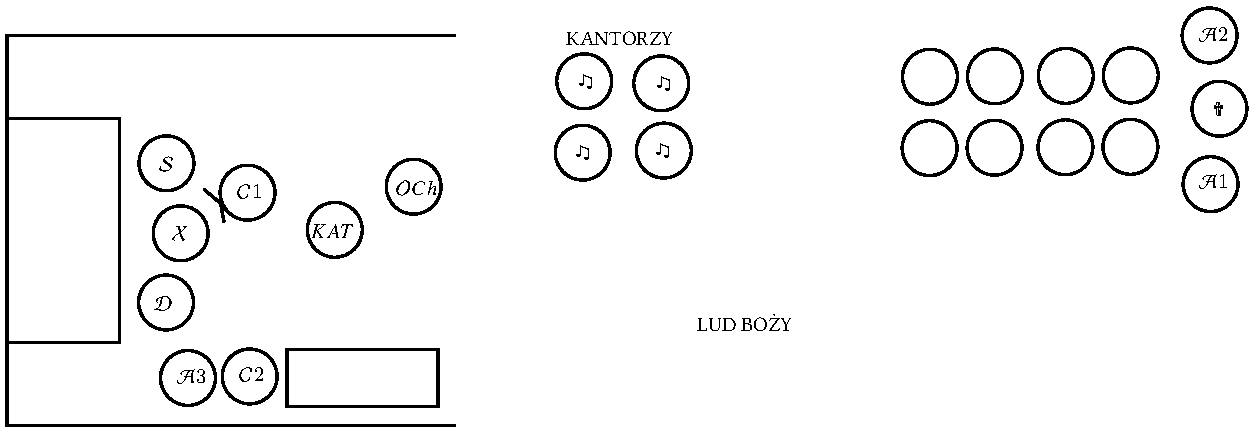
\includegraphics[width=\linewidth]{Figures/Iwo.pdf}
	\caption{Ustawienie ministrantów podczas bierzmowania}
	\label{fig:bierzmowania}
\end{figure}
\subsection{Procesja do ołtarza głównego}
\begin{itemize}
	\item po skończonych obrzędach kantorzy \underline{niezłwocznie} podejmują
	      śpiew \textit{Litanii do Wszystkich Świętych} \footnote{Wszystkie
		      wezwania są śpiewane podwójnie}
	\item \ii~ sprawnie zmienia \textcolor{black!50}{białą kapę i stułę} na
	      \textcolor{violet}{fioletową kapę i stułę}
	\item w międzyczasie \paschal oraz \cc2 przechodzą na początek procesji
	\item procesja idzie tą samą trasą co przyszła do baptysterium
	\item po przybyciu do ołtarza:
	      \begin{itemize}
		      \item \paschal~ i \cc2 odstawiają Paschał na swoje miejsce (czyli
		            na stojak niedaleko stojaka na krzyż procesyjny) przy okazji
		            go gasząc
		      \item \aa\aa~ idą do kredencji
		      \item \ding{63} odkłada krzyż na stojak
		      \item reszta ministrantów idzie do chóru
		      \item \ii, \dd, \ss~ przyklękają oraz ściągają swoje wierzchnie
		            szaty \footnote{Przy stopniach ołtarza} (odpowiednio kapę i
		            plikaty) w czym pomagają \cc1, \cc2 oraz \zz\zz
		      \item \zz\zz~ zabierają szaty do zakrystii
	      \end{itemize}
	\item \ii, \dd, \ss~ kładą się krzyżem na stopniach ołtarza, a wraz z nim
	      klękają wszyscy ministranci (\cc1 z boku \dd)
	\item na wezwanie \sout{Peccatores\dots} \textit{Propitius esto} wszyscy
	      wstają, formuje się procesja \footnote{Nikt nie trzyma nic w rękach, a
		      \ii~ idzie w samej albie i stule} i wychodzi krótką drogą do zakrystii
	\item \ii~ ubiera \textcolor{red}{czerwony ornat, stułę i manipularz}, \dd~
	      ubiera \textcolor{red}{czerwoną dalmatykę, stułę i manipularz},
	      \ss~ ubiera \textcolor{red}{czerwoną tunicellę i manipularz}, a
	      ministranci ubierają koronkowe komże
\end{itemize}
\subsection{Przygotowanie Mszy}
\begin{itemize}
	\item jak ministranci są jeszcze przy chrzcielnicy
	      \begin{itemize}
		      \item dać 3 \textcolor{violet}{fioletowe poduszki} na stopnie
		            ołtarza
		      \item odstawić pulpit do kaplicy
		      \item ustawić relikwie, kwiaty
	      \end{itemize}
	\item po wyjściu \ii~ do zakrystii
	      \begin{itemize}
		      \item \textbf{zapalić 12 świec} (to zrobić jako pierwsze bo
		            najdłużej zajmuje)
		      \item postawić tablice ołtarzowe
		      \item zdjąć {\color{violet} fioletową} zasłonę z antypendium
		            \footnote{Tylko jeśli ludzie mogą oglądać tą zmianę, jeżeli
			            to zbyt skomplikowane, rob icie to w trakcie święcenia
			            wody.}
		      \item odsłonić koronki
	      \end{itemize}
\end{itemize}

